\chapter{Introducción a ROS}
Anteriormente se ha explicado qué es ROS y que características tiene. En este capitulo se pasara a profundizar en su funcionamiento, y mostraremos como se pueden programar los sistemas de paso de mensajes que pasaremos a implementar en un sistema de contenedores Docker.

	\section{Entendiendo ROS}
		
		\subsection{Nodos de ROS}
		
		\subsection{Topics de ROS}
	
	\section{Entorno de trabajo}
	Para poder trabajar con ROS lo primero que debemos tener es un entorno con las herramientas de ROS instaladas. En este caso, como vamos a usar contenedores Docker con todo lo necesario en ellos no necesitaremos instalar ningún tipo de paquete adicional. El Dockerfile que vamos a usar para generar la imagen Ubuntu con ROS ya instalado se encuentra disponible en el Docker Hub y aparece con el nombre \emph{osrf/ros:indigo-desktop}. Esta imagen contiene \cite{ros-installation}:
	\begin{itemize}
		\item \emph{\textbf{ros-base}}, la base de ROS, que a su vez contiene:
		\begin{itemize}
			\item \emph{\textbf{ros-core}}, el núcleo de ROS
			\item Librerías para construir aplicaciones
			\item Librerías para comunicación
		\end{itemize}
		\item \emph{\textbf{rqt}}, framework basado en Qt para construir aplicaciones con interfaz gráfica de usuario (GUI) con ROS
		\item \emph{\textbf{rviz}}, herramienta de visualización 3D para ROS
		\item Librerías genéricas para sistemas robóticos
		
	\end{itemize}
	
	De momento no vamos a hacer uso de ninguna herramienta gráfica. Para probar el funcionamiento de ROS antes de programar sobre nuestro sistema, vamos a elaborar una pequeña aplicación distribuida que nos permita enviar unos datos de un nodo a otro.
	
	\section{Gestionar paquetes ROS}
	Cualquier aplicación que hagamos con ROS será un paquete que podremos instalar. ROS dispone de varias herramientas mediante las cuales crear y compilar esos paquetes. la más famosa de estas herramientas es \emph{\textbf{catkin}}. \emph{catkin} permite crear y compilar paquetes (que se denominan paquetes \emph{catkin}). que contendrán todo el código que desarrollemos. Se basa en el funcionamiento de herramientas como Make o CMake, habituales para compilar aplicaciones en entornos linux.
	
	Para que un paquete se pueda considerar un paquete \emph{catkin} tiene que cumplir una serie de requisitos \cite{ros-catkin-create}:
	
	\begin{enumerate}
		\item El paquete debe contener un fichero de llamado \textit{package.xml} con un formato concreto.
		\begin{itemize}
			\item Este archivo contendrá diferentes metadatos sobre el paquete
		\end{itemize}
		\item El paquete debe contener un fichero \textit{CMakeLists.txt} que usará catkin a la hora de compilar el paquete
		\item No puede haber más de un paquete por carpeta
		\begin{itemize}
			\item No puede haber paquetes anidados en otros paquetes ni varios paquetes en una misma carpeta
		\end{itemize}
	\end{enumerate}
	
		\subsection{Crear paquetes}
		Para crear un paquete con catkin primero debemos crear un workspace de catkin, que es quien contendrá los paquetes que creemos. Lo haremos de la siguiente manera \cite{ros-catkin-workspace}.
		
		\begin{lstlisting}[style=consola,numbers=left]
$ mkdir -p ~/catkin_ws/src
$ cd ~/catkin_ws/src
$ catkin_init_workspace
# Aunque no haya nada compilamos el workspace
$ cd ~/catkin_ws/
$ source devel/setup.bash
		\end{lstlisting}
		
		Una vez creado el workspace podemos crear un paquete de la siguiente manera.
		
		\begin{lstlisting}[style=consola,numbers=left]
$ cd ~/catkin_ws/src
$ catkin_create_pkg paquete std_msgs rospy roscpp
		\end{lstlisting}
		
		Como se puede observar, hemos creado un paquete llamado \textit{paquete}. Los siguientes nombres que le hemos indicado son las dependencia que tiene el paquete, en este caso son dependencias para compilar código fuente de C++ y Python, además de herramientas para manejar mensajes.
		
		\subsection{Compilar paquetes}
		
		Para compilar paquetes generados mediante catkin, se hace uso del comando \emph{catkin-make}. Este comando compila todo en función el archivo \emph{CMakeLists.txt} para saber como debe compilar el paquete.
		
		\begin{lstlisting}[style=consola,numbers=left]
$ cd ~/catkin_ws/
$ catkin_make
		\end{lstlisting}
		
	\section{Modelo distribuido Publisher-Subscriber}
	
	En redes existe un tipo de comunicación conocida como modelo \emph{Publisher-Subscriber}. Esta metodología consiste en dos nodos, uno conocido como \emph{publisher} que va publicando mensajes. Éste nodo no decide a quién se mandan los mensajes, sino que el otro nodo, el nodo \emph{subscriber}, tal y como su nombre indica, se suscribe al nodo que publica los mensajes, y a partir de ese momento recibe los mensajes que va publicando.
	
	En realidad, para separar diferentes tipos de mensajes, se hace uso de \emph{topics} (temas). Esto permite que un publisher pueda tener varios canales de envío de mensajes. Debido a esto, lo que realmente hacen los subscribers es suscribirse a esos topics, y no a los publishers. A su vez, Los publishers deciden en que topic publicar los mensajes.
	
	\begin{figure}[H]
		\centering
		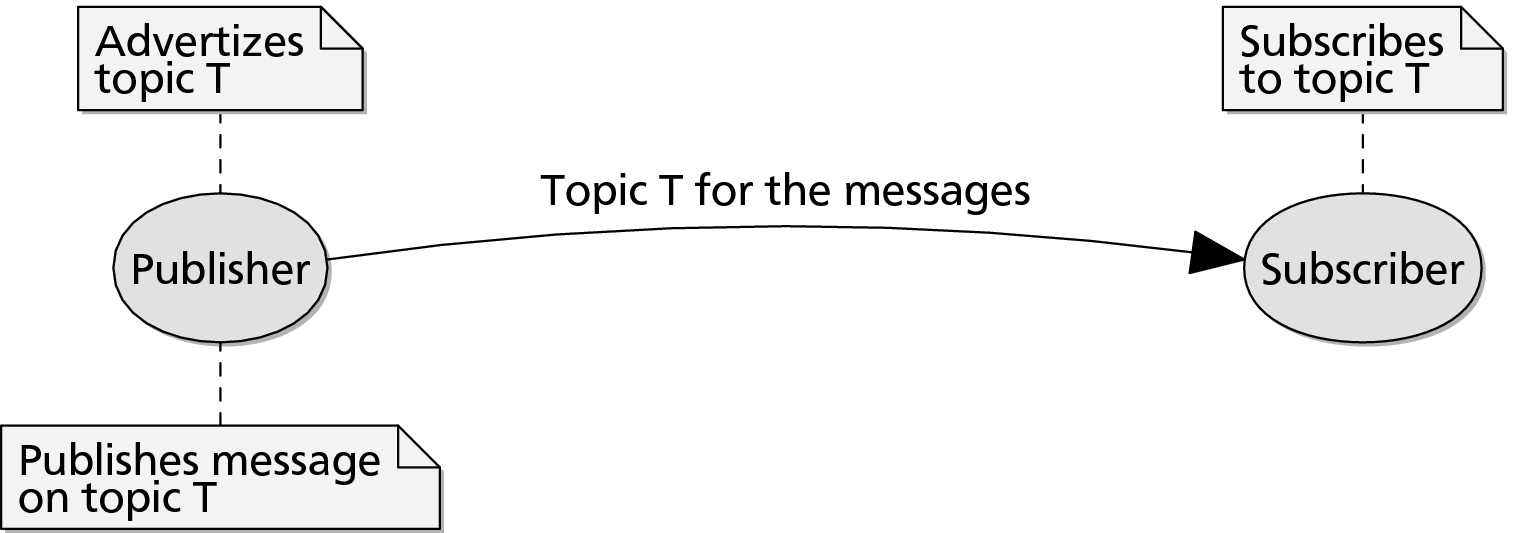
\includegraphics[width=1.0\textwidth]{ros-pub-sub}
		\caption{Modelo Publisher-Subscriber}
		\label{fig:ros-pub-sub}
	\end{figure}